\chapter{AVALIA\c{C}\~AO DO AMBIENTE VIRTUAL DE APRENDIZAGEM}
\label{chap:avaliacao-ambiente-virtual-aprendizagem}
\setcounter{table}{0}

A interface permite o contato dos usu\'arios com o sistema, a qualidade dessa interface est\'a intimamente ligada com o grau de 
satisfa\c{c}\~ao que os usu\'ario venham a ter sobre o sistema. Projetar sistemas adequados ao uso e agrad\'aveis de se utilizar
melhorar\'a a efici\^encia de uso do usu\'ario e agregará mais qualidade ao produto final \cite{antonino2015avaliacao}. 

\citeonline{antonino2015avaliacao} acredita que a utiliza\c{c}\~ao de interfaces que dificultam a execu\c{c}\~ao de tarefas 
pode ser frustrante para o usu\'ario e pode fazer com que ele busque outras op\c{c}\~oes de softwares ou at\'e mesmo crie uma 
rejei\c{c}\~ao ao sistema. 

A qualidade da interface \'e verificada atrav\'es da avalia\c{c}\~ao da usabilidade. Essa técnica utiliza m\'etodos, t\'ecnicas e 
ferramentas, para checar a conformidade de um sistema com os crit\'erios de usabilidade para encontrar problemas de intera\c{c}\~ao e 
corrigi-los \cite{antonino2015avaliacao}. 

\citeonline{nielsen1993usability} divide os critérios básicos de usabilidade em cinco:

\begin{alineascomponto}
	\item \textbf{Facilidade de aprendizado}: O sistema precisa ser fácil de aprender para que o usuário possa explorar de forma agradável as 
funcionalidades do sistema;
	\item \textbf{Eficiência}: O sistema deve ser o mais produtivo possível, possibilitando a execução de tarefas de forma ágil, e sem muito esforço;
	\item \textbf{Memorização}: Mesmo depois de um longo período sem utilizar o sistema, ao retornar, o usuário deve sentir facilidade de uso, sem 
precisar reaprender a usá-lo novamente;
	\item \textbf{Erros}: O sistema precisa ter a menor taxa de erros possível, e caso ocorram é preciso apresentar maneiras simples e rápidas de 
recuperá-los;
	\item \textbf{Satisfação}: A satisfação do usuário determinará o sucesso ou não do sistema. Por isso, quanto mais agradável e prazerosa for à 
experiência dele com o sistema, melhor será o êxito do produto de software.
\end{alineascomponto}

Problemas relacionados a esses crit\'erios de usabilidade, podem dificultar a intera\c{c}\~ao do usu\'ario com o sistema e diminuir a 
qualidade em seu uso. Pensando nisso, realizamos uma avalia\c{c}\~ao de usabilidade no sistema. \citeonline{lima2006ambientecolaborativo} acredita que a avalia\c{c}\~ao de usabilidade tem como objetivos gerais: Validar a eficácia da interação humano-computador face a efetiva realização das tarefas por parte dos usuários; verificar a eficiência desta interação, face os recursos empregados (tempo, quantidade de incidentes, passos desnecessários, 
busca de ajuda, etc.) e; obter indícios da satisfação ou insatisfação (efeito subjetivo) que ela possa trazer ao usuário.

A avaliação do ambiente foi realizada seguindo as seguintes etapas:

\begin{alineascomnumero}
	\item \textbf{Definição do Escopo da Avaliação}: Foram definidos os módulos e interfaces do sistema que seriam objeto da avaliação.
	\item \textbf{Planejamento}: Foram definidas as tarefas que seriam realizadas pelos usuários, assim como as métricas da avaliação, o roteiro da entrevista e a realização de um teste piloto\footnote{Teste realizado preliminarmente em uma escala menor de abrangência, ou seja, menor número de entrevistas, que servirá como orientação para realização da pesquisa propriamente dita, uma vez que fornecerá as devidas correções de questionário, amostra etc.}. 
	\item \textbf{Execução}: Consistiu na utilização de um um método de observação aliado a um método de investigação. Como método de observação, tivemos Testes de Usabilidade, já para o método de investigação contamos com estrevistas.
	\item \textbf{An\'alise dos Resultados}: Foi realizada com o apoio de Gravações de Áudio e Tela obtidas durante a execução dos testes com os usuários.
\end{alineascomnumero}

\section{Definição do Escopo da Avalia\c{c}\~ao}
Como qualquer outro AVA, o ambiente desenvolvido é formado por um conjunto de módulos. Os módulos avaliados são os responsáveis por apresentar as funcionalidades que são acionadas pelos alunos, como visualizar disciplinas, visualizar lições, responder questões, saltar questões, entre várias outras. A seguir, apresentamos o mapa do ambiente com os módulos que fizeram parte do escopo da avaliação:

\begin{figure}[H]
    \centering
    \Caption{\label{fig:mapa_ambiente} Mapa do Ambiente}	
    \UFCfig{}{
	\fbox{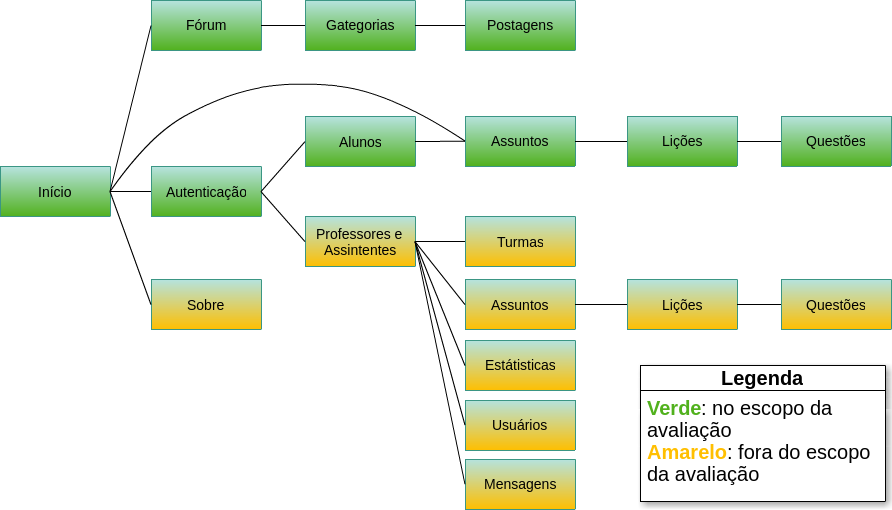
\includegraphics[width=10cm]{figuras/askmath/road_map.png}}
    }{
      \Fonte{Do Próprio Autor}
    }	
\end{figure}

\section{Planejamento}

Durante o planejamento, definimos todos os elementos do plano do teste de usabilidade, tais como os objetivos, métricas, tarefas, entre outros. A seguir, apresentaremos as etapas do planejamento da avaliação.

\subsection{Métricas da Avaliação}

O principal foco dessa avaliação é a usabilidade, por isso, avaliamos alguns fatores
como a facilidade de aprendizado, eficiência no uso, satisfação do usuário, segurança no uso e facilidade de memorização. Na \autoref{tab:metricas_avaliacao}, apresentamos as métricas que foram consideradas durante a avaliação:

\begin{table}[H]
	\Caption{\label{tab:metricas_avaliacao} Métricas para a avaliação}%
	\IBGEtab{}{%

\resizebox{\textwidth}{!}{

\begin{tabular}{|l|l|l|l|l|l|}
\hline
\multicolumn{1}{|c|}{\textbf{Id}} & \multicolumn{1}{c|}{\textbf{Fator}} & \multicolumn{1}{c|}{\textbf{Método de Medição}} & \multicolumn{1}{c|}{\textbf{Nível Ruim}} & \multicolumn{1}{c|}{\textbf{Nível Almejado}} & \multicolumn{1}{c|}{\textbf{Nível Ótimo}} \\ \hline
M1 & Eficiência no uso & \begin{tabular}[c]{@{}l@{}}Tempo gasto para realizar \\ uma tarefa\end{tabular} & \multicolumn{1}{c|}{--} & \multicolumn{1}{c|}{--} & \multicolumn{1}{c|}{--} \\ \hline
M2 & Segurança no uso & \begin{tabular}[c]{@{}l@{}}Número de erros cometidos\\ para cada tarefa\end{tabular} & Por volta de 2 erros & Nenhum erro & Nenhum erro \\ \hline
M3 & Eficiência no uso & \begin{tabular}[c]{@{}l@{}}Número de cliques para \\ realizar uma tarefa\end{tabular} & Por volta de 6 cliques & No máximo 3 cliques & \multicolumn{1}{c|}{--} \\ \hline
M4 & Facilidade de aprendizado & \begin{tabular}[c]{@{}l@{}}Se entende corretamente as \\ informações da interface\end{tabular} & Por volta de 3 perguntas & Sem perguntas & Sem perguntas \\ \hline
M5 & Satisfação do usuário & \begin{tabular}[c]{@{}l@{}}Avaliação do usuário através\\ da entrevista(subjetivo)\end{tabular} & neutro & positivo & muito positivo \\ \hline
\end{tabular}

}

	}{%
	\Fonte{Do Próprio Autor}%
	%\Nota{esta é uma nota, que diz que os dados são baseados na
	%	regressão linear.}%
	%\Nota[Anotações]{uma anotação adicional, seguida de várias outras.}%
}
\end{table}


\subsection{Tarefas}

Após termos o escopo da avaliação e as métricas que seriam utilizadas para avaliar, definimos as tarefas que deveriam ser realizadas pelo usuário durante a avaliação. Confira na tabela a seguir.

\begin{table}[H]
	\Caption{\label{tab:metricas_avaliacao} Tarefas para a avaliação}%
	\IBGEtab{}{%

\resizebox{\textwidth}{!}{

\begin{tabular}{|l|l|}
\hline
\multicolumn{1}{|c|}{\textbf{Id}} & \multicolumn{1}{c|}{\textbf{Tarefa}} \\ \hline
T1 & \begin{tabular}[c]{@{}l@{}}Imagine que você está à procura de uma ferramenta para praticar um pouco dos seus conhecimentos em matemática e \\ acaba de conhecer o AskMath. Para utilizar o sistema pela primeira vez, você deve realizar o seu cadastro.\end{tabular} \\ \hline
T2 & Com o acesso ao sistema, você deve buscar a lição denominada "Introdução a Proposições". \\ \hline
T3 & Após encontrar a lição "Introdução a Proposições", você deve começar a responder as questões apresentadas. \\ \hline
T4 & \begin{tabular}[c]{@{}l@{}}Após resolver algumas questões da lição "Introdução a Proposições", você deve procurar pela disciplina chamada \\ "Diferença".\end{tabular} \\ \hline
T5 & Realize sua inscrição em alguma Turma de Matemática. \\ \hline
T6 & \begin{tabular}[c]{@{}l@{}}Suponha que você ficou com dúvida em algum conteúdo e deseja pedir ajuda. Sendo assim, você deve postar essa \\ dúvida no Fórum de discussões.\end{tabular} \\ \hline
\end{tabular}

}

	}{%
	\Fonte{Do Próprio Autor}%
	%\Nota{esta é uma nota, que diz que os dados são baseados na
	%	regressão linear.}%
	%\Nota[Anotações]{uma anotação adicional, seguida de várias outras.}%
}
\end{table}

Essas tarefas foram escolhidas, pois permitiam o usuário explorar todas as principais funcionalidades do sistemas, assim como suas interfaces. 

\subsection{Roteiro da Entrevista}
Estevistas são uma das técnicas mais utilizadas de coleta de dados e levantamento de requisitos. Trata-se de uma conversa guiada por roteiro de perguntas ou tópicos, na qual o entrevistador busca obter informação de um entrevistado \cite{seidman1998interview}. Existem trêstipos de entrevistas:
\begin{itemize}
	\item \textbf{Estruturadas}: o entrevistador se mantém fiel a um roteiro, fazendo perguntas previamente definidas na ordem especificada. Ele não tem muita liberdade para explorar tópicos novos que surjam durante a entrevista.
	\item \textbf{Não estruturada}:  o entrevistador realiza pergunta de modo flexível, usando perguntas abertas e aprofundando mais em alguns tópicos. O comprometimento do entrevistador é com o tópico abordado.
	\item \textbf{Entrevista semiestruturada}: o roteiro é composto de tópicos ou perguntas (geralmente abertas) que devem ser endereçados na entrevista, em uma ordem lógica. O entrevistador tem liberdade para explorar as respostas e até mesmo modificar a ordem dos tópicos, mas deve manter o foco nos objetivos da entrevista. 
\end{itemize}

Para a avaliação, optamos por utilizar uma estrevista semiestruturada,  por possibilitar uma maior flexibilidade e também uma maior exploração do assunto estudado. Na \autoref{tab:roteiro_entrevista}, apresentamos o roteiro que nos guiou durante as estrevistas.


\begin{table}[H]
	\Caption{\label{tab:roteiro_entrevista} Roteiro para a entrevista}%
	\IBGEtab{}{%

\resizebox{\textwidth}{!}{

\begin{tabular}{|l|l|}
\hline
\multicolumn{1}{|c|}{\textbf{Finalidade}} & \multicolumn{1}{c|}{\textbf{Pergunta}} \\ \hline
\multirow{2}{*}{Caracterização} & Você utiliza regularmente computador? \\ \cline{2-2} 
 & Você já usou algum outro sistema parecido com este? \\ \hline
\multirow{3}{*}{Funcionalidade} & Você acha que o sistema faz o que ele se propõe a fazer? \\ \cline{2-2} 
 & O que você acha das funções do sistema? \\ \cline{2-2} 
 & Tem alguma função que você adicionaria no sistema? \\ \hline
\multirow{2}{*}{Confiabilidade} & Em algum momento o sistema apresentou alguma falha? \\ \cline{2-2} 
 & \begin{tabular}[c]{@{}l@{}}(Caso tenha ocorrido falha). \\ Você acha que o sistema agiu adequadamente na ocorrênciada falha?\end{tabular} \\ \hline
\multirow{4}{*}{Usabilidade} & O que você acha em relação a aprendizagem do uso do sistema? \\ \cline{2-2} 
 & O que você achou do formato dos formulários do sistema? \\ \cline{2-2} 
 & O que você acha das respostas que o sistema de dar quando você executa uma ação? \\ \hline
\multirow{2}{*}{Eficiência} & O que você acha do tempo de resposta do sistema? \\ \cline{2-2} 
 & É fácil encontrar o que se procura no sistema? \\ \hline
\multirow{3}{*}{Melhorias} & O que você não gostou no sistema? \\ \cline{2-2} 
 & O que você gostou no sistema? \\ \cline{2-2} 
 & Qual sugestão de melhoria você daria para o sistema? \\ \hline
\end{tabular}

}

	}{%
	\Fonte{Do Próprio Autor}%
	%\Nota{esta é uma nota, que diz que os dados são baseados na
	%	regressão linear.}%
	%\Nota[Anotações]{uma anotação adicional, seguida de várias outras.}%
}
\end{table}

\subsection{Teste Piloto}

O objetivo do Teste Piloto foi identificar problemas ocasionados por ambiguidades e erros nos materiais de avaliação que poderiam prejudicar a avaliação. Após esse teste, foram realizados correções no roteiro da entrevista e nas tarefas para o teste de usabilidade.

\section{Execução}

Como a abordagem é qualitativa, foram feitos poucos testes, pois o objetivo não é chegar a resultados estatisticamente válidos, mas sim obter evidências ou indicações de problemas e sugestões de como melhorar a qualidade de uso da interface. Tipicamente em testes com usuários se envolve de 5 a 12 usuários \cite{dumas1999practical}. Em nossa avaliação, participaram 6 usuários, que foram escolhidos conforme a definição do público-alvo do ambiente.

Para facilitar a coleta e análise dos dados, gravamos as entrevistas com o auxílio de um gravador e a própria interação do usuário com o sistema através de \textit{softwares} especializados. Ressaltamos que isso só foi possível pois os participantes nos concederam, através de um termo de consentimento livre e esclarecido (\autoref{ap:tcle}), permissão para as gravações. Desde que fosse mantida total confidencialidade dos dados gravados, servido apenas para facilitar sua análise.

A execução do teste consistiu nas seguintes etapas:
\begin{enumerate}
	\item Primeiramente, cada participante foi cumprimentado pelo avaliador e orientado a sentar-se e ficar à vontade. Foi realizado algumas rápidas perguntas curtas para verificar o perfil do participante.
	\item Em seguinda, o avaliador apresentou o propósito e objetivos da avaliação.   
	\item Após as devidas explicações, foi iniciada a realização das tarefas, as quais foram descritas oralmente pelo avaliador. Nesta etapa, o avaliador requisitou que o participante verbalizasse suas dúvidas para ajudar-lo a coletar essas informações.
	\item Depois de concluídas todas as tarefas, o participante foi submetido a uma entrevista, onde o avaliador veio a tratar, além de alguns questionamentos pré-definidos, fatos ocorridos durante a realização das tarefas.
	\item Após a entrevista, o entrevistador agradeceu ao participante e lhe entregou um brinde como forma de agradecimento.  
\end{enumerate}

\section{An\'alise dos Resultados}

\subsection{Tempo de execução das tarefas}
Na \autoref{tab:execucao_tarefas} apresentamos as medidas de tempo de execução das seis tarefas realizadas comparando-as com valores previamente estabelecidos: nível ruim, almeijado e ótimo.


\begin{table}[H]
	\Caption{\label{tab:execucao_tarefas}  Tempo de Execução das Tarefas}%
	\IBGEtab{}{%

\resizebox{\textwidth-8cm}{!}{

\begin{tabular}{|l|c|c|c|c|c|c|}
\hline
\multicolumn{1}{|c|}{\textbf{\begin{tabular}[c]{@{}c@{}}Tarefas/\\ Participantes\end{tabular}}} & \textbf{T1} & \textbf{T2} & \textbf{T3} & \textbf{T4} & \textbf{T5} & \textbf{T6} \\ \hline
Participante 1 & 103s & 20s & - & 5s & 5s & 47s \\ \hline
Participante 2 & 126s & 9s & - & 175s & 7s & 34s \\ \hline
Participante 3 & 78s & 10s & - & 35s & 5s & 55s \\ \hline
Participante 4 & 48s & 5s & - & 30s & 5s & 40s \\ \hline
Participante 5 & 90s & 5s & - & 11s & 4s & 35s \\ \hline
Participante 6 & 35s & 9s & - & 20s & 8s & 25s \\ \hline
\textbf{Média} & \textbf{80s} & \textbf{9s} & \textbf{-} & \textbf{46s} & \textbf{5s} & \textbf{39s} \\ \hline
Nível ruim & 120 & 30s & - & 100s & 15s & 60s \\ \hline
Nível almeijado & 45s & 5s & - & 10s & 5s & 30s \\ \hline
Nível ótimo & 20s & 2s & - & 4s & 3s & 15s \\ \hline
\end{tabular}

}
}{%
	\Fonte{Do Próprio Autor}%
	\Nota{Os dados estão expressos em segundos}
	\Nota{Não é correto calcular o tempo de realização da atividade T3, já que isso depende do nível de conhecimento dos participantes com o conteúdo apresentado}
	%\Nota[Anotações]{uma anotação adicional, seguida de várias outras.}%
}
\end{table}

Em geral, o tempo de execução das tarefas foi maior que o nível almeijado, isso pode indicar que a eficiência no uso do sistema pode está comprometida. Em especial, nas tarefas T1 e T4, o tempo para execução dessas tarefas são bem maiores do que o nível almeijado, em alguns casos, até o dobro do tempo. Com isso, podemos concluir que a eficiência de uso para realizar um cadastro e buscar uma lição específica está abaixo do nível desejado.  

\subsection{Número de erros cometidos na execução das tarefas}
Na \autoref{tab:erros_cometidos_tarefas} apresentamos as medidas de número de erros cometidos durante a execução das seis tarefas, comparando-as com valores previamente estabelecidos: nível ruim, almeijado e ótimo. 

\begin{table}[H]
	\Caption{\label{tab:erros_cometidos_tarefas}  Número de Erros Cometidos}%
	\IBGEtab{}{%

\resizebox{\textwidth-8cm}{!}{

\begin{tabular}{|l|c|c|c|c|c|c|}
\hline
\multicolumn{1}{|c|}{\textbf{\begin{tabular}[c]{@{}c@{}}Tarefas/\\ Participantes\end{tabular}}} & \textbf{T1} & \textbf{T2} & \textbf{T3} & \textbf{T4} & \textbf{T5} & \textbf{T6} \\ \hline
Participante 1 & 1 & 1 & 0 & 0 & 0 & 0 \\ \hline
Participante 2 & 1 & 1 & 0 & 4 & 0 & 0 \\ \hline
Participante 3 & 0 & 0 & 0 & 1 & 0 & 0 \\ \hline
Participante 4 & 0 & 0 & 0 & 1 & 0 & 0 \\ \hline
Participante 5 & 0 & 0 & 0 & 0 & 0 & 0 \\ \hline
Participante 6 & 0 & 0 & 0 & 1 & 0 & 0 \\ \hline
\textbf{Média} & \textbf{0.16} & \textbf{0.33} & \textbf{0} & \textbf{1.16} & \textbf{0} & \textbf{0} \\ \hline
Nível ruim & 2 & 2 & 2 & 2 & 2 & 2 \\ \hline
Nível almeijado & 0 & 0 & 0 & 0 & 0 & 0 \\ \hline
Nível ótimo & 0 & 0 & 0 & 0 & 0 & 0 \\ \hline
\end{tabular}

}
	}{%
	\Fonte{Do Próprio Autor}%
	%\Nota{esta é uma nota, que diz que os dados são baseados na
	%	regressão linear.}%
	%\Nota[Anotações]{uma anotação adicional, seguida de várias outras.}%
}
\end{table}

Em relação ao número de erros cometidos durante a realização das tarefas, foram poucos. Somente o Participante 2 durante a realização da tarefa T4 que acabou cometendo muito mais erros do que o nível almeijado. Mas como ele acabou encontrando uma outra forma alternativa de realizar a tarefa (usando a barra de busca), isso pode ser relevado. Dessa forma, podemos concluir que o sistema possui uma boa segurança no uso nesse quesito. 

\subsection{Número cliques realizados na execução das tarefas}
Na \autoref{tab:cliques_realizados_tarefas} apresentamos as medidas de número de cliques durante a execução das seis tarefas realizadas, comparando-as com valores previamente estabelecidos: nível ruim, almeijado e ótimo. 

\begin{table}[H]
	\Caption{\label{tab:cliques_realizados_tarefas}  Número de Cliques Realizados}%
	\IBGEtab{}{%

\resizebox{\textwidth-8cm}{!}{

\begin{tabular}{|l|c|c|c|c|c|c|}
\hline
\multicolumn{1}{|c|}{\textbf{\begin{tabular}[c]{@{}c@{}}Tarefas/\\ Participantes\end{tabular}}} & \textbf{T1} & \textbf{T2} & \textbf{T3} & \textbf{T4} & \textbf{T5} & \textbf{T6} \\ \hline
Participante 1 & 3 & 4 & 2 & 4 & 3 & 4 \\ \hline
Participante 2 & 5 & 3 & 2 & 7 & 3 & 4 \\ \hline
Participante 3 & 3 & 2 & 2 & 4 & 3 & 4 \\ \hline
Participante 4 & 3 & 2 & 2 & 4 & 3 & 4 \\ \hline
Participante 5 & 3 & 2 & 2 & 3 & 3 & 4 \\ \hline
Participante 6 & 3 & 2 & 2 & 4 & 3 & 4 \\ \hline
\textbf{Média} & \textbf{3.33} & \textbf{0.33} & \textbf{2} & \textbf{4.33} & \textbf{3} & \textbf{4} \\ \hline
Nível ruim & 6 & 6 & 6 & 6 & 6 & 6 \\ \hline
Nível almeijado & 3 & 3 & 3 & 3 & 3 & 3 \\ \hline
Nível ótimo & 3 & 2 & 2 & 3 & 3 & 3 \\ \hline
\end{tabular}

}
	}{%
	\Fonte{Do Próprio Autor}%
	%\Nota{esta é uma nota, que diz que os dados são baseados na
	%	regressão linear.}%
	%\Nota[Anotações]{uma anotação adicional, seguida de várias outras.}%
}
\end{table}

Apesar do tempo de realização das tarefas serem maior do esperado, a quantidade cliques realizados para completar as tarefas foram próxima do nível almeijado, o que indica que os participantes levaram mais tempo buscando entender a interface do que tomando caminhos alternativos para alcançar seus objetivos.

\subsection{Número de perguntas realizadas durante a execução das tarefas}
Durante a entrevista, não foram feitas muitas perguntas por parte dos participantes. Apenas o Participante 2 na Tarefa 4, que após tentar realizar a atividade por um tempo, questionou o avaliador se poderia usar a barra de busca para achar a lição ao qual a tarefa proponha.

\subsection{Resultados da Entrevista}

\begin{itemize}
	\item Você utiliza regularmente computador? \\
	Para esta pergunta, cinco participantes responderam que sim, apenas o Participante 3 respondeu que não usa tão constantemente.
	\item Você já usou algum outro sistema parecido com este? \\	
	Dois seis participantes, apenas um respondeu que já usou um sistema parecido, mas que já fazia muito tempo e não recordava o nome.
	\item Você acha que o sistema faz o que ele se propõe a fazer? \\
	Todos responderam que sim. Quando questionado, o Participante 1 respondeu: ''Sim, gostei muito da ideia e gostaria de usar depois''.
	\item O que você acha das funções do sistema? \\
	Todos dissetam que das que viram, gostaram. O Participante 5 disse ainda: ``Acho que ainda tem poucas funcionalidades, mas talvez isso possa deixar mais fácil pra gente usar''.
	\item Tem alguma função que você adicionaria no sistema? \\
	As funções citadas pelos participantes foram: Bate-papo entre os alunos, um sistema de Ranking e videoaulas dos conteúdos. 
	\item Em algum momento o sistema apresentou alguma falha? \\
	Nenhum dos participante relatou falhas do sistema durante seu uso.
	\item Você acha que o sistema agiu adequadamente na ocorrênciada falha? \\
	Não foi realizada, já que de acordo com os participantes, o sistema não apresentou falhas.
	\item O que você achou da execução das funções do sistema? \\
	Todos gostaram das funções, apenas o Participante 4 que relatou uma dificuldade em buscar uma lição especifica que acabou ficando fácil com o uso da barra de buscar.
	\item O que você acha em relação a aprendizagem do uso do sistema? \\
	Em geral, os participantes respoderam que por ter poucas funcionalidades, foi fácil aprender a utilizar o sistema. 
	\item O que você achou do formato dos formulários do sistema? \\
	Nessa pergunta, todos respoderam que acharam normais. O participante 6 relatou: ``É bem padrão, acho que não deve ser mudado''.
	\item O que você acha do tempo de resposta do sistema? \\
	Todos relataram que o tempo de resposta do sistema foi rápido.
	\item É fácil encontrar o que se procura no sistema? \\
	Alguns dos participantes relataram uma certa dificuldade em encontrar um lição específica.
	\item O que você não gostou no sistema? \\
	Os participantes informaram que não teve algo que eles não gostaram no sistema.
	\item O que você gostou no sistema? \\
	Dois participantes disseram que gostaram da opção de poder saltar uma pergunta, um deles falou sobre a descrição das perguntas que segundo ele "estão bem explicadas", e dois gostaram das lições possuirem níveis e do sistema de pontuação.
	\item Qual sugestão de melhoria você daria para o sistema? \\
	Nessa pergunta, os participante voltaram a falar na adição de mais funcionalidades ao sistema, como bate-papo, ranking e a adição de conteúdos em vídeo.
\end{itemize}